\documentclass{beamer}
\usetheme{metropolis} % Use metropolis theme
\usepackage{lmodern}

\renewcommand{\footnoterule}{%
  \hspace{2cm}
  \kern -3pt
  \hrule width \textwidth height 1pt
  \kern 2pt
}
\usepackage[utf8]{inputenc}
\usepackage[T1]{fontenc}
\usepackage[autostyle, english = british]{csquotes}
\usepackage[british]{babel}
\usepackage{todonotes}
\usepackage[%
  backend=biber,
  doi=false,
  url=false,
  isbn=false,
  eprint=false,
  style=verbose,
  citestyle=verbose,
  hyperref=true,
  maxnames=99,
  minnames=1,
  maxbibnames=99,
  firstinits,
  uniquename=init]{biblatex}
%\DeclareFieldFormat[inproceedings, article]{pages}{}%
%\DeclareFieldFormat[inproceedings]{organization}{}%
  % ignore some field for citations
\DeclareSourcemap{
  \maps[datatype=bibtex, overwrite]{
    \map{
      \step[fieldset=edition, null]
      \step[fieldset=publisher, null]
      \step[fieldset=pages, null]
      \step[fieldset=organization, null]
    }
  }
}

\addbibresource{../bibliography.bib}

\let\oldfootnotesize\footnotesize
\renewcommand*{\footnotesize}{\oldfootnotesize\fontsize{6}{6}}

\usepackage{caption}
\usepackage{xpatch}
\usepackage{xcolor}
\usepackage{bm}
\usepackage{amsmath}
\usepackage{mathtools} % for \mathclap
\usepackage{varioref}
\usepackage{siunitx}
\usepackage{hyperref}
\usepackage[noabbrev]{cleveref}
\newcommand{\creflastconjunction}{, and\nobreakspace} % use Oxford comma
\usepackage{todonotes}
\usepackage{multimedia}

\graphicspath{{../figures/}}
\newcommand{\Qrho}{\ensuremath{\rho}}
\newcommand{\Qj}{\ensuremath{\rho \bm{v}}}
%\newcommand{\Qv}{\ensuremath{\Qrho^{-1} \Qj}}
\newcommand{\Qv}{\ensuremath{\bm{v}}}
\newcommand{\QE}{\ensuremath{\rho E}}
\newcommand{\stressT}{\ensuremath{\bm{\sigma}}}
\newcommand{\pressure}{\ensuremath{p}}
\newcommand{\maxConvEigen}{\ensuremath{\vert \lambda_c^{\text{max}} \vert}}
\newcommand{\maxViscEigen}{\ensuremath{\vert \lambda_v^{\text{max}} \vert}}

\newcommand{\cn}{\footnote{\enquote{TODO: Citation.}, 2017, \textbf{Conference}, \textit{Author 1, Author 2, Author 3, Author 4} }}

\title{Cloud Supercomputing with the ExaHyPE-Engine\\Master Thesis Kick-Off}
\author{Lukas Krenz\\Adviser: Leonhard Rannabauer\\Supervisor: Prof.\ Dr.\ Michael Bader}
\date{October 18, 2018} 
\institute{\textsc{tum}, Chair for Scientific Computing}

\begin{document}
\maketitle
\begin{frame}{Rising Bubble: Hydrostatic Equilibrium\footfullcite{robert1993bubble}}
  \begin{columns}
    \begin{column}[t]{0.5\textwidth}
      \begin{itemize}
      \item 
  Air is in hydrostatic equilibrium:

  Gravitational force and pressure-gradient force are \textbf{exactly balanced}.

  \item Constant potential temperature (temperature normalized by pressure) with slightly warmer bubble.
        
  \end{itemize}
    \end{column}~%
    \begin{column}[t]{0.5\textwidth}
      \begin{figure}[h]
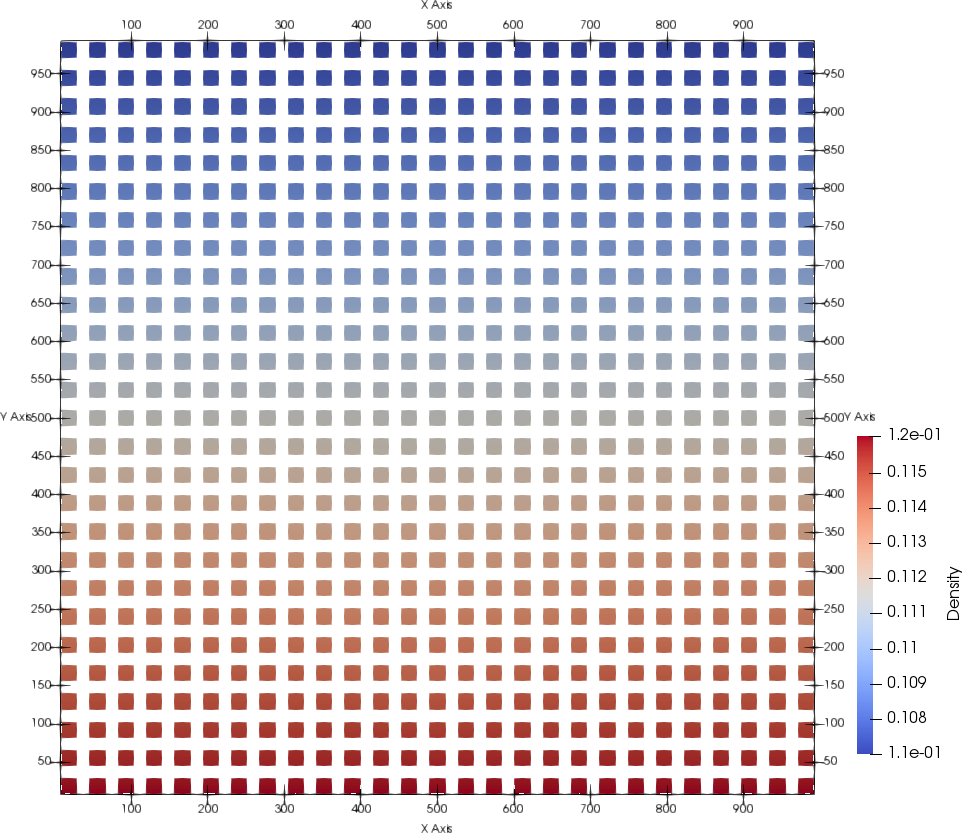
\includegraphics[width=1.0\textwidth]{hydrostatic_density}
\caption{Density in equilibrium}
\end{figure}
    \end{column}
  \end{columns}
\end{frame}

\begin{frame}
  \frametitle{Rising Bubble: Simulation}
   \begin{figure}[h]
    \centering
    \movie[width=0.9735\textwidth, height=0.55\textwidth, autostart,, loop, poster]{}{bubbles_order1.ogv}
    \caption{Rising bubble scenario}
  \end{figure}
\end{frame}

\begin{frame}{The ADER-DG Approach\footfullcite{dumbser2008unified}}
  Solve \textbf{hyperbolic conservation laws} of the form
\begin{equation}
  \label{eq:conservation-law}
 \frac{\partial}{\partial_t}  Q + \nabla \cdot F(Q) = S(\bm{x}, t, Q)
\end{equation}
with $Q$ vector of conserved variables, $\bm{x}$ position, $t$ time,  $\nabla \cdot F(Q)$ divergence of flux and $S(\bm{x}, t, Q)$ source term.

\textbf{Discontinuous Galerkin} (\textsc{DG}) divides domain into disjoint elements, approximates solutions by piecewise-polynomials.
Elements are connected by solving the Riemann problem.

\textbf{ADER}-Approach uses space-time polynomials for time integration instead of Runge-Kutta procedures.

Implemented in the \textsc{PDE}-Framework \textbf{ExaHyPE}.
\end{frame}

\begin{frame}{The Navier-Stokes Equations}
  Vector of conserved quantities:
\begin{equation}
  \label{eq:conserved-variables}
 Q = \left( \Qrho, \Qj, \QE \right) 
\end{equation}
With $\Qrho$ density of fluid, $\Qj$ velocity density and $\QE$ energy density.

Flux:
\begin{equation}
  F(Q, \textcolor{orange}{\nabla Q}) = 
  \begin{pmatrix}
    \Qj \\
    \Qv  \otimes \Qj + \bm{I} \pressure + \textcolor{orange}{\stressT (Q, \nabla Q)}  \\
    \Qv \cdot \left(\bm{I} \QE + \bm{I} \pressure + \textcolor{orange}{\stressT (Q, \nabla Q)} \right) -
    \textcolor{orange}{\kappa \nabla T}
  \end{pmatrix}
\end{equation}

$T$ temperature, $\pressure$ pressure,
$\textcolor{orange}{\stressT}$ stress tensor, $\textcolor{orange}{\kappa \nabla T}$ heat diffusion term
\end{frame}

\begin{frame}{Problem: Not hyperbolic}
  \textsc{DG} solves equations of the form (e.g.\ Euler):
  \begin{equation}
  \label{eq:conservation-law}
 \frac{\partial}{\partial_t}  Q + \nabla \cdot F(Q) = S(\bm{x}, t, Q)
\end{equation}

We have:
\begin{equation}
  \label{eq:conservation-law}
 \frac{\partial}{\partial_t}  Q + \nabla \cdot F(Q, \textcolor{orange}{\nabla Q}) = S(\bm{x}, t, Q)
\end{equation}

\textbf{Solution}:
Modify numerical flux (Riemann solver), time step size (\textsc{cfl}-Condition) and boundary conditions to \textbf{allow diffusive terms}\footfullcite{dumbser2010arbitrary}.

\alert{No explicit discretization} of gradient $\nabla Q$.
\end{frame}

\begin{frame}{Current status}
  \begin{block}{Working}
  \begin{itemize}
  \item Numerical scheme
  \item Cloud scenario
  \end{itemize}
  \end{block}

  \begin{block}{Goals}
  \begin{itemize}
  \item Fix convergence
  \item Adaptive Mesh Refinement
  \item Finite Volume Limiting\footfullcite{dumbser2016simple}
  \item Coupling of Navier-Stokes with other PDE (e.g.\ simple advection equation) by solving Riemann problem at boundary
  \end{itemize}
  \end{block}
\end{frame}

\begin{frame}{Current status of Convergence-Tests}
  \begin{figure}[h]
    \centering
   \includegraphics[width=0.8\textwidth]{{l2_error}}
    \caption{Mesh-Size vs $L_2$ error }
    \label{fig:l2-error}
  \end{figure}
\end{frame}

\begin{frame}{Summary}
  \begin{block}{Main Objectives}
  \begin{itemize}
  \item \textbf{Navier-Stokes equations} can describe dynamics of clouds.
  \item \textbf{ADER-DG} can be used to discretize Navier-Stokes equations.
  \item The \textbf{ExaHyPE-Engine} provides an efficient, scalable implementation of ADER-DG scheme. 
  \end{itemize}
  \end{block}

  \begin{block}{Bonus Objectives}
    \begin{itemize}
    \item All \textbf{extensions} to engine (diffusive fluxes, coupling) useful for \textbf{other users} of ExaHyPE.
    \item First use of ExaHyPE-Engine for \textbf{simulation of clouds}.
    \end{itemize}

  \end{block}
\end{frame}

\end{document}